\documentclass[10pt,a4paper]{standalone}
\usepackage{tikz}
\usetikzlibrary{trees}

\begin{document}
\usetikzlibrary{trees}
% First, set the overall layout of the tree
% You might need to play with these sizes to ensure nothing overlaps.
\tikzstyle{level 1}=[level distance=1.5cm, sibling distance=3cm]
\tikzstyle{level 2}=[level distance=1.5cm, sibling distance=1.5cm]
\tikzstyle{level 3}=[level distance=1.5cm, sibling distance=1cm]
\tikzstyle{level 4}=[level distance=1.5cm, sibling distance=2cm]
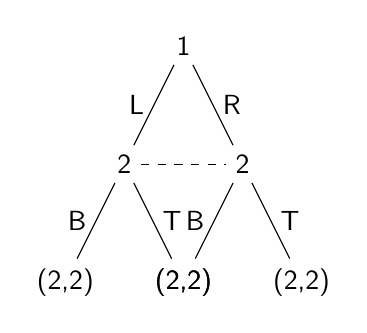
\begin{tikzpicture}[font=\sffamily]
%Start with the parent node, and slowly build out the tree
% with each "child" representing a new level of the diagram
% each "node" represents a labelled (or unlabeled if you
% want) node in the diagram.
\node {1}
    child{
                        %Put the name of the node in parenthesis for
                        % reference later. The label shown in the diagram
                        % goes in the brackets. This label can use math mode.
            node(a){2}
            child{
                node(a1){(2,2)}
                edge from parent
                node[left]{B}
             }
             child{
                node(a2){(2,2)}
                edge from parent
                node[right]{T}
             }
             edge from parent
             node[left]{L}
    }
    child{
             node(b){2}
            child{
                node(b1){(2,2)}
                edge from parent
                node[left]{B}
             }
             child{
                node(b2){(2,2)}
                edge from parent
                node[right]{T}
             }
     		edge from parent
     		node[right]{R}
    };
%Now I create the information set. Note that I utilize the names
% that I had previously assigned to nodes in my graph
\draw [dashed](a)--(b);
\end{tikzpicture}
\end{document}